% !TEX root = ../thesis_main.tex
%
%
%%% 
\begin{figure}[h!!t]
	\centering
	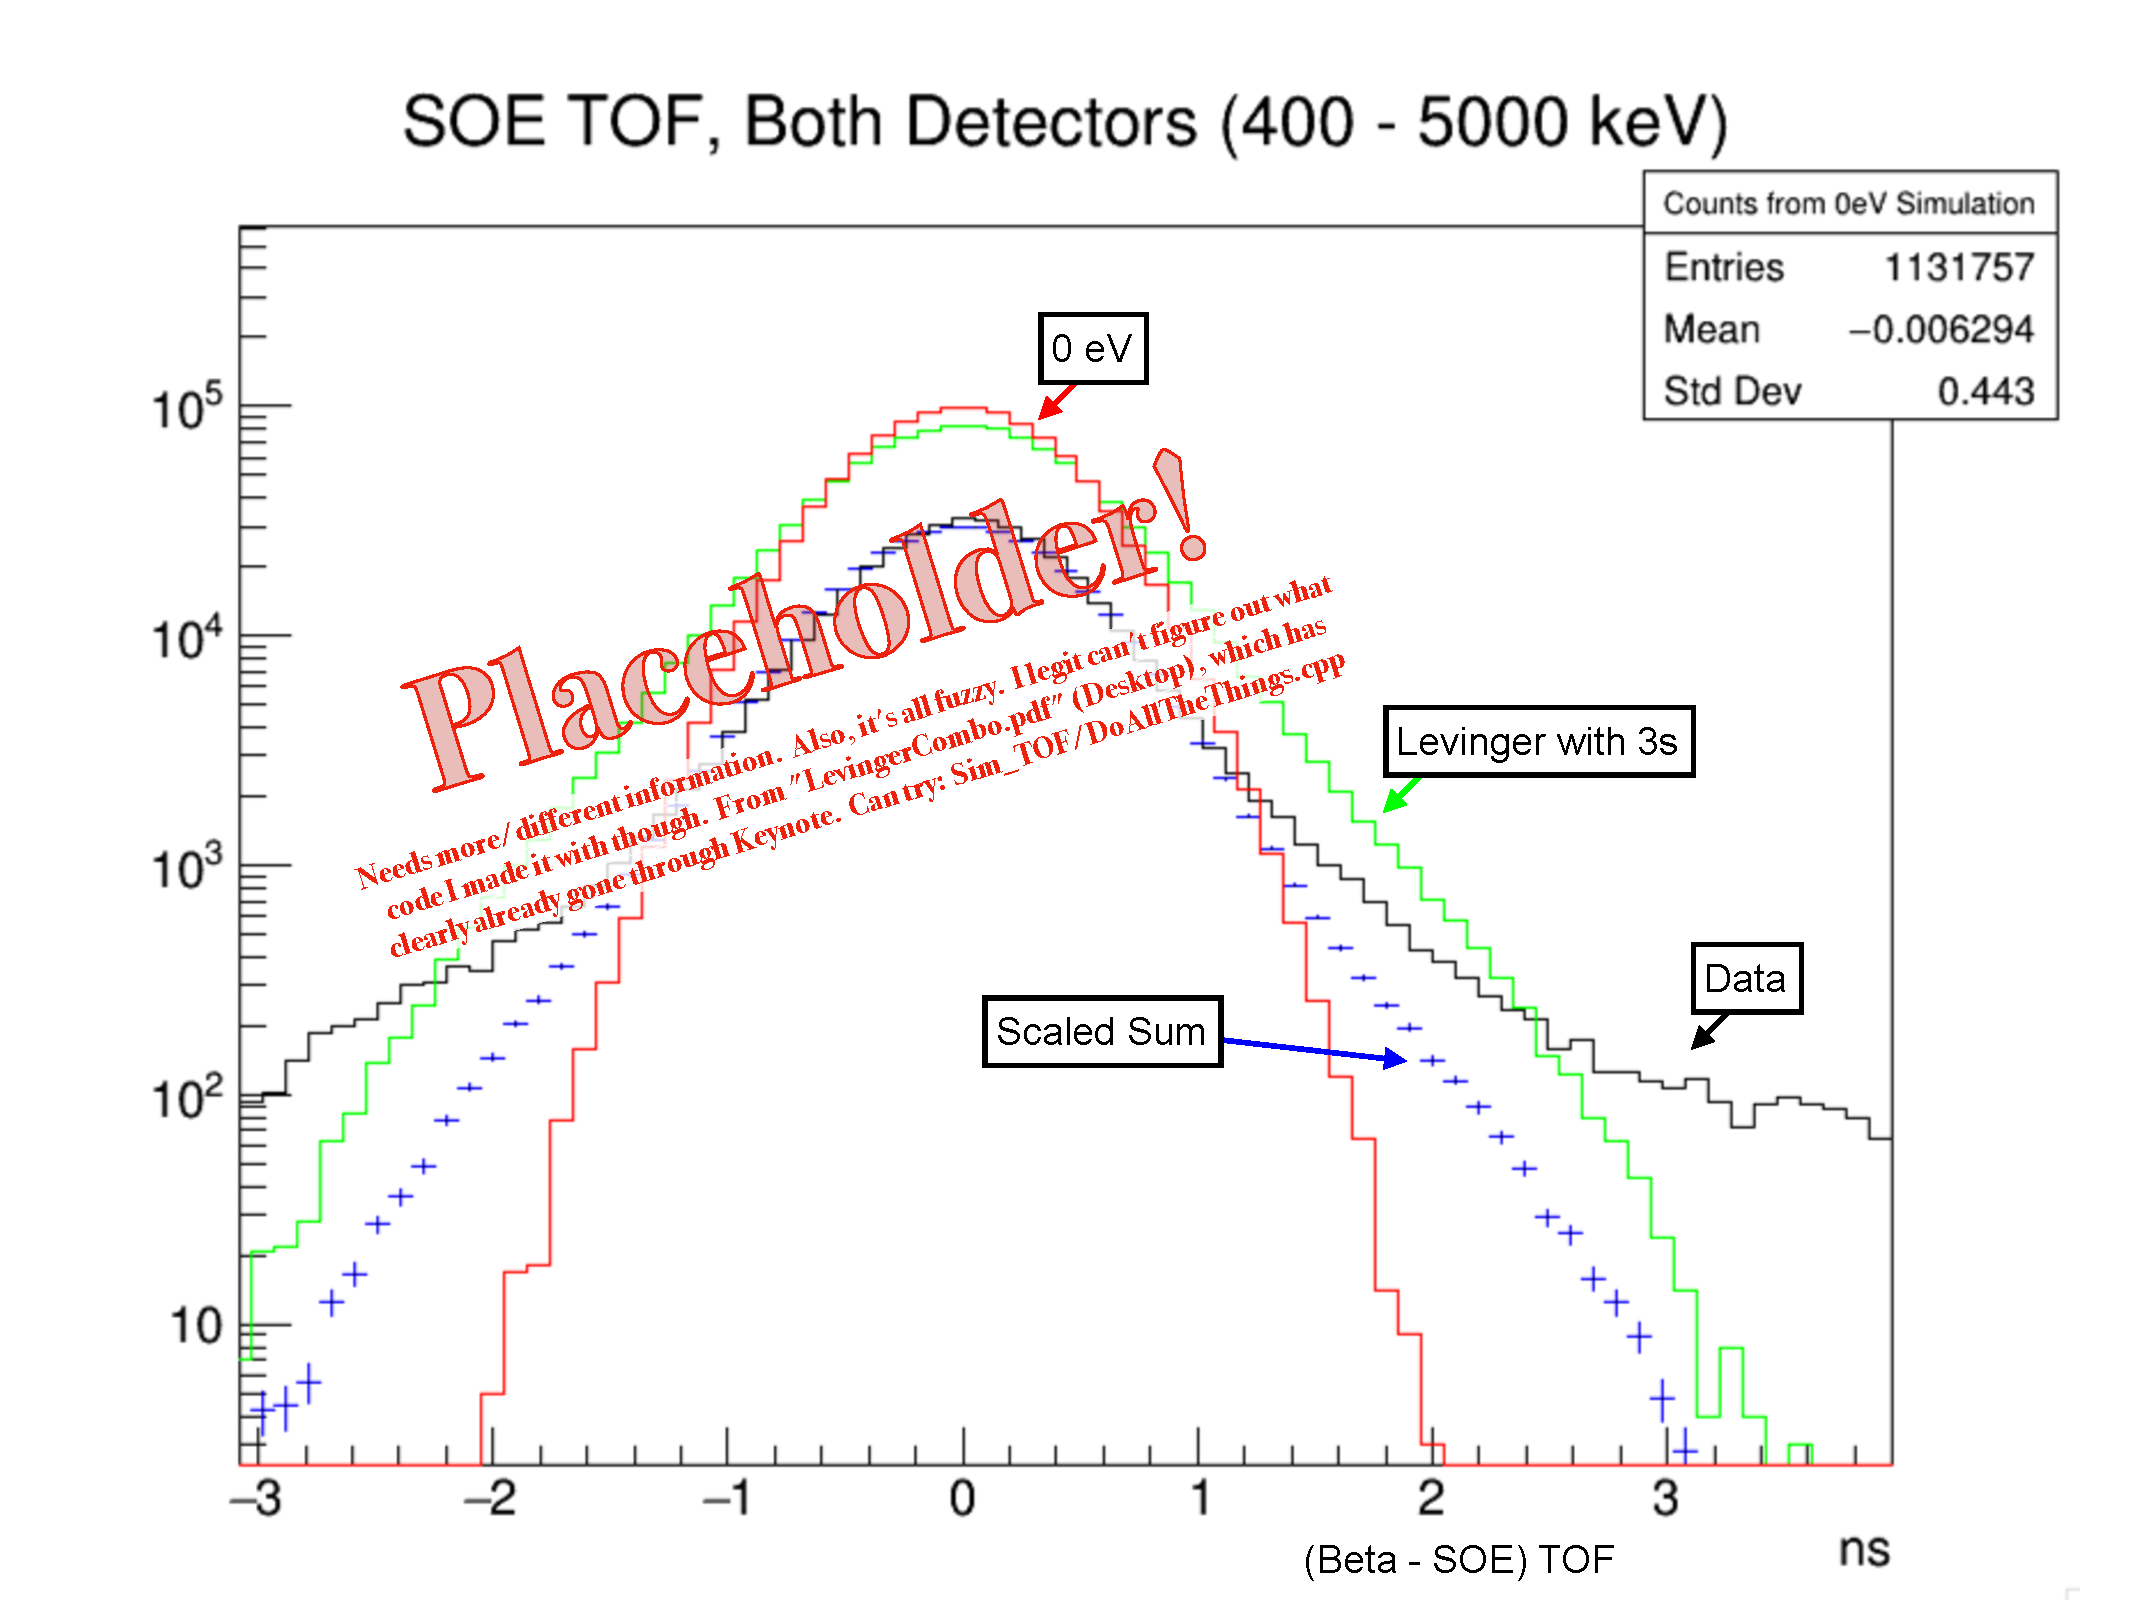
\includegraphics[width=.999\linewidth]
	{Figures/Levinger_SOETOF_prelim.pdf}
	\caption[Levinger TOF]{Shake-off electron TOF (w.r.t. beta TOA) spectrum, showing how the spectrum is different if one includes different sets of initial electrons to be shaken off.  I forget why some of them have 0 eV.  Maybe those are the ones from the $\isotope[37]{Ar}^+$. ... Levinger TOF spectra for some different sets of SOE initial orbitals before shake-off.  (At least that's what it's supposed to be, after I fix the picture).  It's reconstructed event-by-event with beta times-of-flight that would pass some basic `good event' cuts.  Anyway, it turns out, it doesn't much matter what orbitals you lose SOEs from.  That's nice.  In the end, I used 85+15.  \comment{(Need to re-plot this.)} }	
	\label{fig:levinger_TOF}
\end{figure}
